%% Standard-Vorspann
\documentclass[a4paper,11pt,oneside]{article}
\usepackage{ngerman}                   
\usepackage[utf8]{inputenc}
\usepackage[T1]{fontenc}
\usepackage[fleqn]{amsmath}

%% Auf Schriftart Palatino umschalten
\usepackage{mathpazo}
\usepackage[scaled=.95]{helvet}
\usepackage{courier}

%% fast immer benoetigte Pakete
\usepackage{epsfig}
\usepackage{amssymb}
\usepackage{alltt}
\usepackage{latexsym}
\usepackage{makeidx}
\usepackage{textcomp}
\usepackage{rotating}
\usepackage{color}
\usepackage{caption}
\usepackage{verbatim}
\usepackage{fancyhdr}

%packages for codelisting see: http://stackoverflow.com/questions/741985
\usepackage{color, xcolor}
\usepackage{listings}
\usepackage{courier}

\usepackage[
  plainpages=false,
  unicode=true,          % non-Latin characters in Acrobat?s bookmarks
  pdftitle=,
  pdfauthor=GSM OpenBTS Handover Action Group,
  pdftoolbar=true,        % show Acrobat?s toolbar?
  pdfmenubar=true,        % show Acrobat?s menu?
  pdffitwindow=true,     % window fit to page when opened
  pdfstartview={FitV},    % fits the width of the page to the window
  pdfnewwindow=true,      % links in new window
  colorlinks=true,       % false: boxed links; true: colored links
  linkcolor=red,          % color of internal links
  citecolor=green,        % color of links to bibliography
  filecolor=magenta,      % color of file links
  urlcolor=cyan,          % color of external links
  hyperfootnotes=false,
  bookmarks,
]{hyperref}

%Konfigutation für Codelisting
%see: http://stackoverflow.com/questions/741985
\lstset{
	basicstyle=\footnotesize\ttfamily, % Standardschrift
	numbers=left,               % Ort der Zeilennummern
	numberstyle=\tiny,          % Stil der Zeilennummern
	numbersep=5pt,              % Abstand der Nummern zum Text
	tabsize=2,                  % Groesse von Tabs
	extendedchars=true,         %
	breaklines=true,            % Zeilen werden Umgebrochen
	stringstyle=\ttfamily, % Farbe der String
	showspaces=false,           % Leerzeichen anzeigen ?
	showtabs=false,             % Tabs anzeigen ?
	xleftmargin= 17pt,
	framexleftmargin=17pt,
	framexrightmargin=5pt,
	framexbottommargin=4pt,
	showstringspaces=false      % Leerzeichen in Strings anzeigen ?        
}
\lstloadlanguages{PHP, XML, HTML}
\DeclareCaptionFont{white}{\color{white}}
\DeclareCaptionFormat{listing}{\colorbox[cmyk]{0.43, 0.35, 0.35,0.01}{\parbox{\textwidth}{\hspace{15pt}#1#2#3}}}
\captionsetup[lstlisting]{format=listing,labelfont=white,textfont=white, singlelinecheck=false, margin=0pt, font={bf,footnotesize}}

\newcommand{\utsection}[2]{%Section mit Untertitel (ut)
    \section[#1]{#1\newline\normalfont\small\textit{Von: #2}}
}
\newcommand{\utsubsection}[2]{%Subsection mit Untertitel (ut)
    \subsection[#1]{#1\newline\normalfont\small\textit{Von: #2}}
}	
		
%% spezielles Zeug
\usepackage{Abschlussarbeit}

%% Index erzeugen
\makeindex

%% jetzt geht's los
\begin{document}
\raggedbottom

% Vorspann der Arbeit
%
\begin{titlepage}
\begin{flushright}
\includegraphics[width=70mm]{img/hm}%
\end{flushright}

\vspace*{20mm}
\begin{center}
{\Large Hochschule München}\\
{\large Fakultät für Mathematik und Informatik}\\

\vspace*{15mm}
{\huge Projektdokumentation Mobile Netze}\\

\vspace*{10mm}
{\huge \bfseries{Handover mit OpenBSC und OpenBTS}} \\
\vspace*{15mm} 
\end{center}

\vspace*{30mm}

\begin{tabular}{lll}
\textbf{\large {Autoren:}} & & \large {Max Eschenbacher, B.Eng.}\\
			   & & \large {Stefan Giggenbach, B.Eng.}\\
			   & & \large {Thomas Waldecker, B.Eng.}\\
& & \\

\textbf{\large {Abgabe:}} & & \large {19.03.2012}\\
& & \\

\textbf{\large {betreut von:}} & & \large {Prof. Dr. Alf Zugenmaier}\\
& & \\
\end{tabular}

\end{titlepage}

%% Inhaltsverzeichnis
\tableofcontents
\newpage

\utsection{Einleitung}{Stefan Giggenbach}

Im Rahmen des Moduls Mobile Netze im Masterstudiengang Informatik wird mit der Durchfürhung einer Projektarbeit, dass in der Vorlesung vermittelte Wissen vertieft und um praktische Aspekte ergänzt. In der vorliegenden Projektarbeit wurde die Handover-Funktionalität in einem GSM-Netzwerk untersucht. In diesem Kapitel wird nach einer theoretischen Einführung in die GSM-Handover-Thematik das Projektziel und die entsprechende Vorgehensweise beschrieben.

\subsection{GSM-Handover}\label{sec:handover}

Der Handover stellt in einem GSM-Netzwerk eine wichtige Aufgabe des Mobility Management dar. Ändert ein Teilnehmen bei aktiver Verbindung seinen Standort, ist es möglich das er den von einer Funkzelle abgedeckten Bereich verlässt. In einem solchen Fall wird die Verbindung durch den Wechsel (Handover) zu einer angrenzenden Nachbarzelle aufrecht erhalten. Grundsätzlich unterscheidet man in einem GSM-Netzwerk folgende Handoverszenarien \cite{bib:grundkursmks}:

\begin{itemize}
 \item Intra BSC Handover
 \item Inter BSC Handover
 \item Inter MSC Handover
 \item Subsequent MSC Handover
\end{itemize}

Die Unterschiede in den Abläufen der einzelnen Szenarien werden in \cite{bib:grundkursmks} ausführlich beschrieben. Aus Sicht der Mobile Station unterscheiden sich die genannten Handoverszenarien nicht. Im folgenden werden nur die Abläufe des Intra BSC Handover beschrieben, die für das Verstädnis der Arbeit entscheidend sind.

Während einer aktiven Verbindung wird der BSC in regelmäßigen Zeitäbständen über die Signalqualität im Up- bzw. Downstream informiert. Zu diesem Zweck sendet die Mobile Station über den SACCH sogenannte Measurement Reports, die anschließend im BSC zur Bestimmung der Downstream-Signalqualität ausgewertet werden. In den Measurement Reports sind neben Messergebnissen zur aktuell verwendeten BTS auch Messergebnisse zu benachbarten BTS, die auf Anweisung des BSC während den Sendepausen von der Mobile Station ermittelt werden. Die Signalqualität des Upstreams wird durch Messergebnisse aus der entsprechenden BTS ebenfalls im BSC berechnet. Der BSC kann aufgrund der eingehenden Measurement Reports zu dem Ergebnis kommen, dass ein Handover zwischen zwei benachbarten BTS notwendig ist, um einen Abbruch der Verbindung zu verhindern.

\begin{figure}[h!]
  \centering
  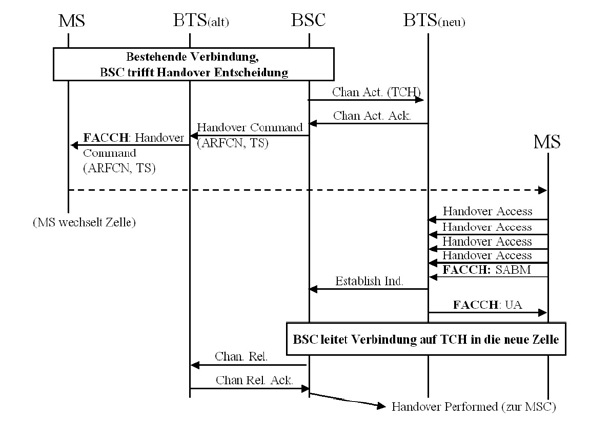
\includegraphics[width=0.85\textwidth]{img/handover.png}
  \caption{Ablaufdiagramm eines Handover \cite{bib:grundkursmks}}
  \label{fig:adhandover}
\end{figure}

Abbildung \ref{fig:adhandover} zeigt den Ablauf eines Handover nach der Entscheidung eines BSC. Im ersten Schritt wird ein TCH in der neuen BTS aufgebaut. War dieser Vorgang erfolgreich, wird der Mobile Station über den FACCH der bestehenden Verbindung ein Handover Command übermittelt. Das Handover Command enthält als wichtige Parameter die Frequenz und den Timeslot des TCH der neuen BTS. Nach der Synchronisation der Mobile Station mit der neuen BTS, sendet es in vier aufeinanderfolgenden Bursts eine Handover Access Message und anschließend eine Set Asynchronous Balanced Mode Message. Die neue BTS quittiert den erfolgreichen Handover mit einem Established Indicator gegenüber dem BSC und einer UA Massage gegenüber der Mobile Station. Nachdem der BSC die Verbindung auf den neuen TCH umschaltet, wird der TCH in der alten BTS abgebaut. Der Handover Vorgang ist damit abgeschlossen.

Die wichtigesten Punkte für die Analyse bzw. Impelmentierung einer Handover-Funktionalität sind damit:

\begin{itemize}
 \item Erfassung und Auswertung der Measurement Reports
 \item Logik für die Entscheidungsfindung eines Handover
 \item Inter BTS Kommunikation zum Aufbau neuer TCH
 \item Erzeugen und Senden eines Handover Command
 \item Umschalten der bestehenden Verbindung und Abbau des alten TCH
\end{itemize}

\subsection{Projektziel und -durchführung}

Ziel der Projektarbeit ist die Integration der in Abschnitt \ref{sec:handover} eingeführten Handover-Funktionalität in die Opensource Software OpenBTS. Das OpenBTS Projekt ermöglicht, zusammen mit einer entsprechenden Radio-Hardware und zusätzlichen Software-Komponenten (GNURadio und Asterisk), den Betrieb eines kompletten GSM-Netzwerks. Mit der kommerziell vertriebenen Version der Software ist bereits ein Handover zwischen zwei BTS möglich. Die Vorraussetzungen für eine erfolgreiche Integration eines Handover-Moduls sind somit gegeben. Die Architektur und Inbetriebnahme des verwendeten OpenBTS-Systems werden in Kapitel \ref{sec:openbts} ausführlich behandelt.

Vor der Integrations- und Implementierungsphase wird der Ablauf eines Handover genauer analysiert. Zu diesem Zweck wird ein OpenBSC-System aufgesetzt, mit dem das in Abschnitt \ref{sec:handover} beschriebene Handoverszenario reproduziert werden kann. Der Aufbau, die Inbetriebnahme und die Konfiguration des OpenBSC-Systems für die Durchführung eines Intra BSC Handover wird in Kapitel \ref{sec:openbsc} behandelt. Die anschlißende Analyse der durchgeführten Handover erfolgt mit Hilfe der auf der Um- und Abis-Schnittstelle erstellen Wireshark Traces und ist in Abschnitt \ref{sec:analyse} beschrieben.

Der Architekturentwurf für die Integration und die teilweise durchgeführte Implementierung des Handover-Moduls werden in Kapitel \ref{sec:hom} behandelt. Der erreichte Projektstand und geschaffene Ansatzpunkte für weitere Projektarbeiten an der Integration des Handover-Moduls schließen die Arbeit ab.



\utsection{OpenBSC}{Stefan Giggenbach}\label{sec:openbsc}

\subsection{Überblick}

Bei OpenBSC handelt es sich wie bei OpenBTS um ein Open Source Projekt. Die Entwicklung erfolgt vollständig in der Sprache C und hat keinen direkten Bezug zum OpenBTS Projekt. Der große Vorteil von OpenBSC liegt in der \textit{network in the box} (nitb) genannten Version, die ohne zusätzliche Software-Komponenten den Betrieb eines GSM-Netzwerks ermöglicht. Mit OpenBSC wird zu einem sehr frühen Zeitpunkt im Projekt ein GSM-Netzwerk mit Handover-Funktionalität betrieben mit dem die entsprechenden Abläufe analysiert werden können (siehe Kapitel \ref{sec:analyse}).

\begin{figure}[h!]
  \centering
  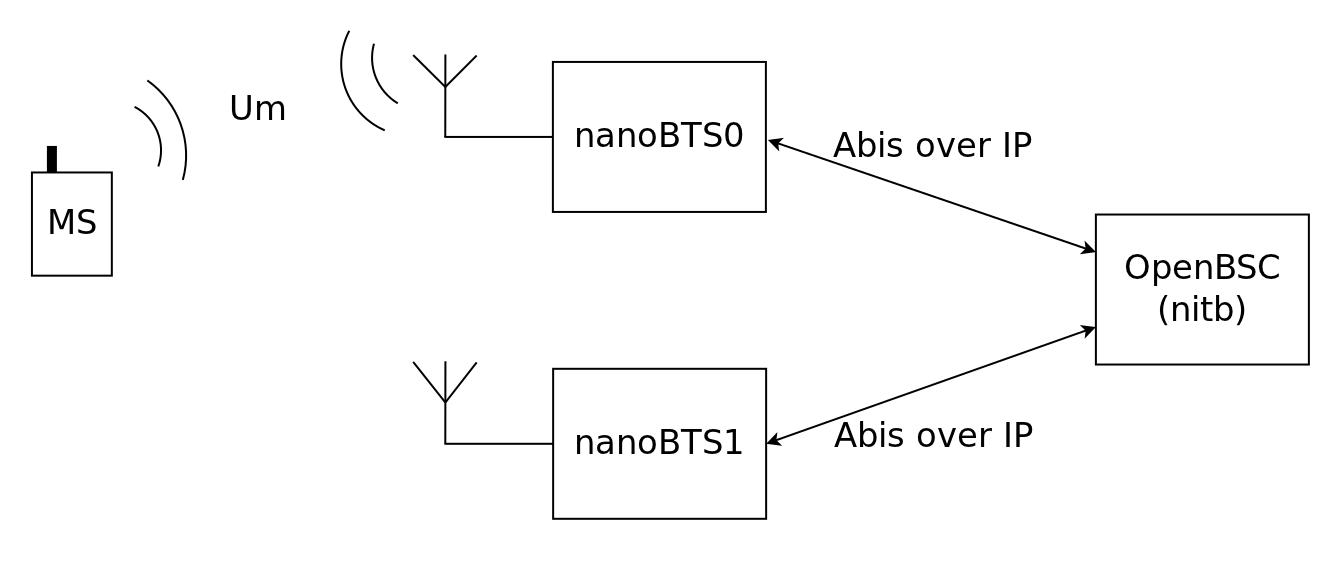
\includegraphics[width=0.9\textwidth]{img/openbscarch}
  \caption{OpenBSC Versuchsaufbau}
  \label{fig:openbscarch}
\end{figure}

Abbildung \ref{fig:openbscarch} zeigt den im Projekt verwendeten Versuchsaufbau. OpenBSC übernimmt nicht nur die Aufgaben des BSC, sondern auch die des MSC. Die Teilnehmerdatenbanken HLR und VLR werden mit einer SQLite3 Datenbank realisiert. Wie in Abbildung \ref{fig:openbscarch} dargestellt, werden zwei nanoBTS der Firma ip.access verwendet. Diese werden über getrennte Abis-over-IP-Schnittstellen an OpenBSC angebunden. Mit dem dargestellten Versuchsaufbau ist somit die Durchführung eines in Abschnitt \ref{sec:handover} beschriebenen Intra BSC Handover mit verhältnismäßig geringem Installations- und Konfigurationsaufwand möglich.

\subsection{Installation und Konfiguration}

Die Installation von OpenBSC ist ausführlich im Wiki des Projekts \cite{bib:buildopenbsc} dokumentiert. In diesem Abschnitt werden nur die wichtigsten Punkte der Installation und die Konfiguration des Systems für den Multi-BTS-Betrieb behandelt.

OpenBSC (nitb) besteht aus insgesamt drei Komponenten:

\begin{itemize}
 \item \textit{libosmocore} - Die Kernbibliothek, die auch für andere Projekte (z.\,B. OsmoBTS) verwendet wird.
 \item \textit{libosmo-abis} - Die Bibliothek zur Umsetzung der Abis- und Abis-over-IP-Schnittstellen.
 \item \textit{openbsc} - Die eigentliche OpenBSC-Software, welche auch die nitb Version enthält.
\end{itemize}

Nach der Kompilierung und Installation dieser drei Komponenten können die beiden nanoBTS, die sich im selben IP-Netzwerk befinden müssen, konfiguriert werden. Dazu werden die zwei Anwendungen \lstinline{./ipaccess-find} und \lstinline{./ipaccess-config} im Verzeichnis \lstinline{<openbsc>/src/ipaccess} benötigt. Die Verwendung der beiden Anwendungen und die benötigten Parameter zur Konfiguration werden ebenfalls im Wiki des Projekts \cite{bib:ipaccess} erläutert. Die bei der Konfiguration der nanoBTS vergebene UnitID wird dabei für die im Folgenden beschriebene Konfiguration von OpenBSC benötigt.

Um den Betrieb beider nanoBTS und die Handover-Funktionalität von OpenBSC zu aktivieren, muss die Konfigurationsdatei von OpenBSC modifiziert werden. Als Grundlage wird die Beispielkonfiguration \lstinline{<openbsc>/doc/examples/osmo-nitb/nanobts/openbsc.cfg} verwendet. Listing \ref{lst:config} zeigt auszugsweise die wichtigsten Inhalte der modifizierte Konfigurationsdatei.

\begin{lstlisting}[label=lst:config,caption=OpenBSC Konfigurationsdatei (Auszug)]
!
! OpenBSC (0.10.1.40-2935) configuration saved from vty
.
network
 network country code 262
 mobile network code 98
 .
 handover 1
 .
 bts 0
  type nanobts
  band DCS1800
  cell_identity 0
  .
  ip.access unit_id 42 0
  .
  trx 0
   rf_locked 0
   arfcn 846
   nominal power 23
   max_power_red 22
   .
 bts 1
  type nanobts
  band DCS1800
  cell_identity 1
  .
  ip.access unit_id 43 0
  .
  trx 0
   rf_locked 0
   arfcn 867
   nominal power 23
   max_power_red 22
   .
\end{lstlisting}

Neben dem Network Country Code und dem Mobile Network Code (Zeilen 5 und 6) muss in den Netzwerkeinstellungen die Handover-Funktionalität gesetzt werden (Zeile 8). Die Konfiguration der beiden nanoBTS beschränkt sich im Wesentlichen auf die Vergabe der eindeutigen CellIDs (Zeilen 13 und 26), der vorher festgelegten UnitIDs (Zeilen 15 und 28) und den beiden Frequenzen (ARFCN in Zeilen 19 und 32).

Nach der Modifikation der Konfigurationsdatei wird diese im Verzeichnis \lstinline{<openbsc>/src/osmo-nitb} gespeichert. Anschließend kann das System mit dem Befehl \lstinline{./openbsc} im selben Verzeichnis gestartet werden. Die Bedienung von OpenBSC erfolgt nach dem Start über eine Telnetsitzung auf Port 4242. Mit Hilfe des Command Line Interfaces der Telnetsitzung ist auch die Administration der Teilnehmerdatenbank möglich. Die Verwendung des CLI ist aufgrund der interaktiven Eingabe selbsterklärend.

Um einen Handover auszulösen, kann bei aktiver Verbindung entweder die Position einer Mobile Station verändert werden oder die Signalqualität wird durch entsprechende Schirmung der Geräte in ausreichendem Umfang reduziert. Die Analyse der mit OpenBSC durchgeführten Handover wird in Kapitel \ref{sec:analyse} detailliert beschrieben.

%\section{OpenBTS}
\utsection{OpenBTS}{Max Eschenbacher}\label{sec:openbts}
\textbf{OpenBTS (Open Base Transceiver Station)} ist eine freie Unix-Applikation die in C++ entwickelt wurde. Mit Hilfe eines Software Radios und der entsprechenden Hardware, kann OpenBTS die GSM Luftschnittstelle \textit{Um} simulieren. In Verbindung mit einer Private Branch Exchange (PBX) können die Mobilfunkteilnehmer untereinander, sowie, je nach Anbindung, mit VoIP- bzw. Festnetzteilnehmern telefonieren.

\subsection{Aufbau und Zusammenspiel}
\subsubsection{Komponenten}
Ein funktionsfähiges OpenBTS System besteht aus folgenden Komponenten:

\begin{itemize}
\item \textbf{OpenBTS}\\
Die eigentliche Kernsoftware, welche (fast) den gesamten GSM-Stack oberhalb des Radios realisiert.
\end{itemize}
\begin{itemize}
\item \textbf{Transceiver}\\
Kombination aus Radio-Hardware (USRP1) und der ansprechenden Software (GNUradio). Dadurch wird der gesamte Physical Layer der GSM \textit{Um} Luftschnittstelle realisiert. Die eingesetzte Universal Software Radio Peripheral (USRP) ist von der Firma Ettus Research (siehe Abbildung \ref{fig:usrp1}) und wird über einen FA-Synthesizer (siehe Abbildung \ref{fig:fasyn}) mit 52MHz betrieben.
\begin{figure}[htbp]
  \centering
  \begin{minipage}[b]{6cm}
    \centering
    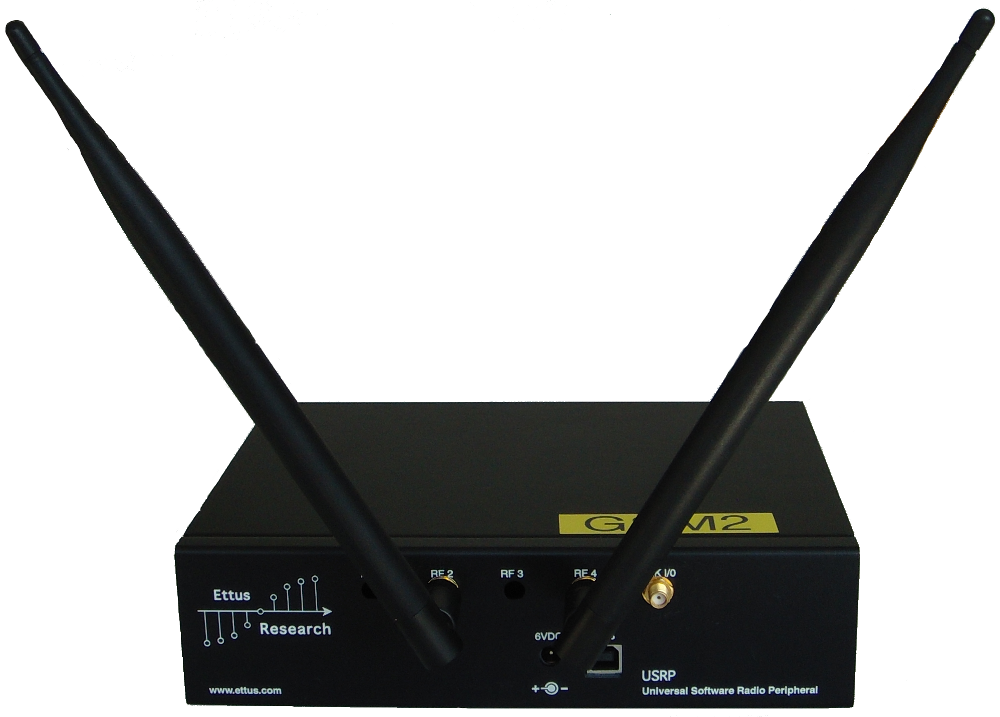
\includegraphics[width=1.00\textwidth]{img/usrp1.png}
    \caption{GSM-Radio USRP1}
	\label{fig:usrp1}
  \end{minipage}
  \begin{minipage}[b]{2cm}
  \end{minipage}
  \begin{minipage}[b]{6cm}
    \centering
    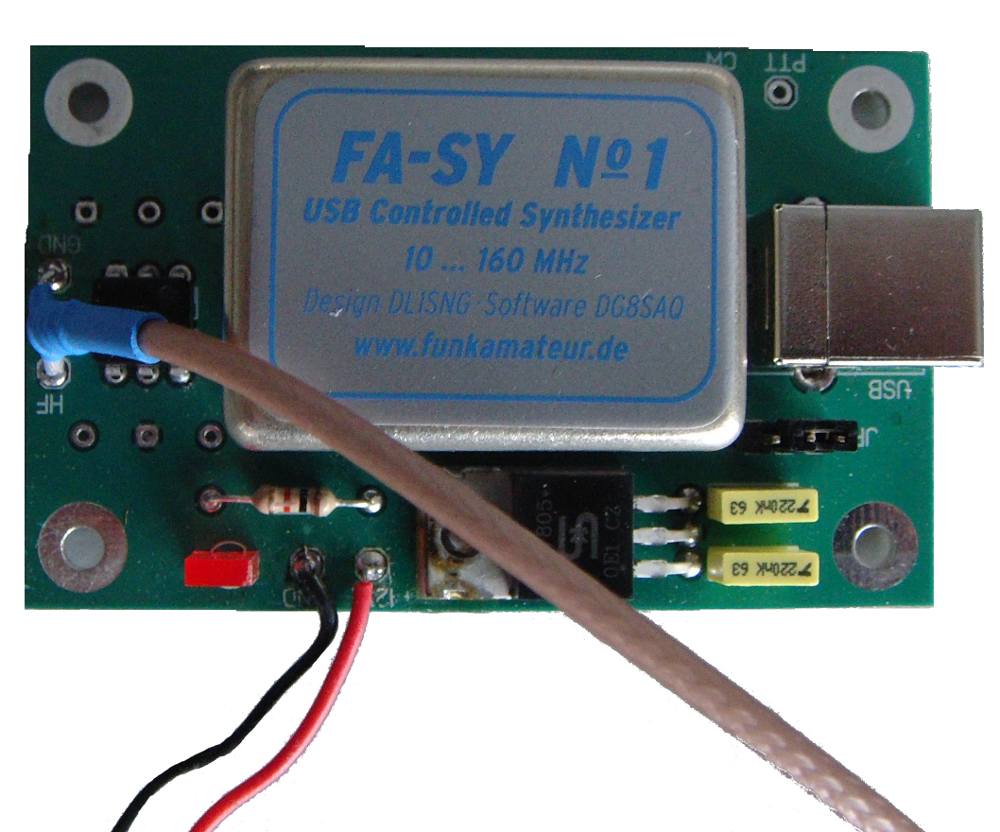
\includegraphics[width=0.50\textwidth]{img/frequenzgen.png}
    \caption{FA-Synthesizer}
	\label{fig:fasyn}
  \end{minipage}
\end{figure}
\end{itemize}
\begin{itemize}
\item \textbf{Asterisk}\\
OpenBTS benutzt eine herkömmliche PBX um die Gesprächsvermittlung zu realisieren und damit das klassische Mobile Switching Center (MSC) zu ersetzen. Wir setzen dabei die freie Software namens Asterisk ein die in OpenBTS unterstützt wird und neben der Hauptaufgabe, der Gesprächsvermittlung, weitere Features wie beispielsweise Mailbox-Services enthält. 
\end{itemize}
\begin{itemize}
\item \textbf{Smqueue}\\
Smqueue ist für den Versand bzw. die Speicherung von SMS Nachrichten zuständig. Darüber hinaus verfügt es über "`Short Code"'-Funktionalität, die es erlaubt den Inhalt von Textnachrichten als Eingabeargumente für selbst entwickelte lokale Anwendungen zu benutzen oder an eine E-Mail-Adresse weiterzuleiten.
Smqueue hat bereits eine solche Short-Code-Anwendung namens "`register"' integriert. Hierbei handelt es sich um eine interaktive Registrierung, bei der der Benutzer eine SMS mit der gewünschten Rufnummer als Inhalt an die BTS sendet. Wird diese Nummer noch nicht verwendet, trägt "`register"' diese zusammen mit der IMSI in die Subscriber Registry ein. %\footnote{Die interaktive Registrierung wurde von uns nicht getestet.}
\end{itemize}
\begin{itemize}
\item \textbf{Subscriber Registry}\\
Die Subscriber Registry ist eine Datenbank die OpenBTS für die Subscriber Informationen nutzt. Sie ersetzt zum einen das klassische GSM Home Location Register (HLR) und zum anderen die SIP Registry von Asterisk.
\end{itemize}

\textit{(Die Komponenten Smqueue und Subscriber Registry (sipauthserve) sind keine eigenständigen Projekte, sondern Bestandteile von OpenBTS.)}\\

In Abbildung \ref{fig:openbts_comp} sind die Beziehungen, sowie die Verbindungsprotokolle der einzelnen Komponenten untereinander ersichtlich.
\newpage
\begin{figure}[htbp]
	\centering
		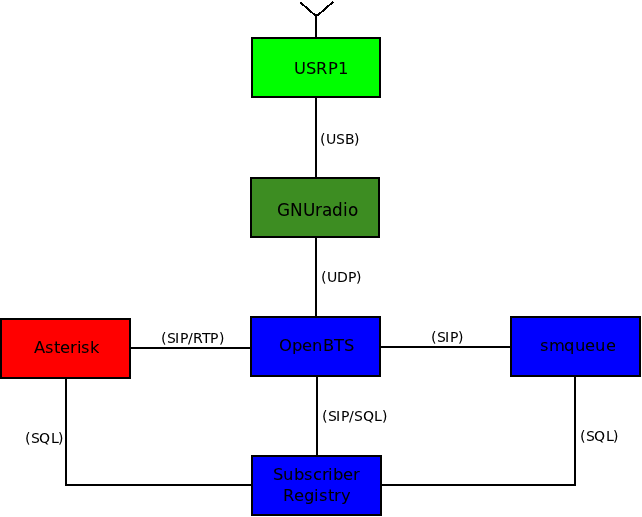
\includegraphics[width=0.80\textwidth]{img/openbts_comp.png}
	\caption{Systemkomponenten}
	\label{fig:openbts_comp}
\end{figure}


In Abbildung \ref{fig:openbts_system_diagram} ist noch einmal der Kommunikationsfluss im Hinblick auf SIP aufgezeichnet. Dabei kennzeichnen die \textbf{schwarzen} Pfeile SIP-Verbindungen, die \textcolor{red}{\textbf{roten}} Pfeile Datenbankabfragen und der \textcolor{blue}{\textbf{blaue}} Pfeil ODBC-Verbindungen.

\begin{figure}[hbtp]
	\centering
		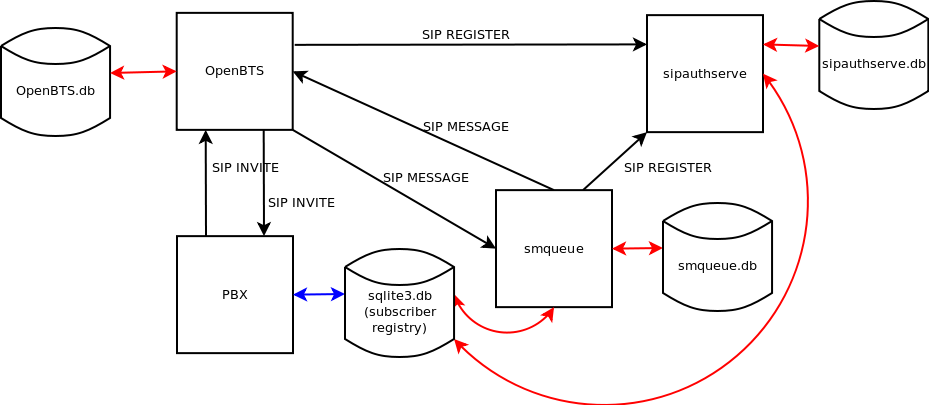
\includegraphics[width=1.00\textwidth]{img/openbts_system_diagram.png}
	\caption{System Diagramm (Quelle: \cite{bib:diagramm:openbts})}
	\label{fig:openbts_system_diagram}
\end{figure}
\subsubsection{Datenbanken}
Im System Diagramm findet man vier Datenbanken vor, welche für folgende Zwecke benutzt werden:

\begin{table}[h]
	\centering
		\begin{tabular}{ll}
			\textbf{OpenBTS.db} & Alle Konfigurationsparameter von OpenBTS werden\\
			& seit der Version P2.8 nicht mehr in einzelnen Konfi-\\
			& gurationsdateien hinterlegt, sondern in einer zentra-\\
			& len SQL-Datenbank verwaltet.\\
			\textbf{sipauthserve.db} & Hier werden die angemeldeten MS-Teilnehmer\\
			& registriert.\\
			\textbf{sqlite3.db} & Von Asterisk benutzte Datenbank zur SIP User\\ 
			& Registrierung, dessen Einträge von "`sipauthserve"'\\
			& erzeugt werden.\\
			 \textbf{smqueue.db} & Enthält alle Konfigurationsparameter von smqueue.\\
		\end{tabular}
\end{table}

\subsubsection{GSM/SIP-Abläufe}
\label{gsmsip} 
Einer der Hauptmerkmale von OpenBTS ist es, dass Mobile Switching Center (MSC) durch einen herkömmlichen VoIP-Switch (Asterisk) zu ersetzen. Dabei ist jede MS aus Sicht des Asterisk-Servers ein SIP-Endpunkt. Dieser SIP-Endpunkt wird von OpenBTS realisiert und verwaltet. Dabei wird jeder MS ein eigener SIP-Benutzername in der Form "`IMSIxxxxxxxxxxxxxxx"' zugeordnet, wobei die "`x"' der IMSI-Nummer der MS entsprechen. Die IP-Adresse jedes SIP-Endpunktes ist immer die gleiche und zwar die der BTS, also dort wo der OpenBTS-Dienst läuft. OpenBTS ist gegenüber Asterisk transparent, d.h. Asterisk sieht nur die MS als SIP-Endpunkte. Eine aktive Sprachverbindung besteht in diesem Kontext somit aus zwei Teilstrecken. Einmal die Strecke Asterisk $ \longleftrightarrow $ OpenBTS, in der SIP/RTP-Pakete die Sprachübertragung erledigen, und zum anderen die Strecke OpenBTS $ \longleftrightarrow $ MS, bei der ein GSM Sprach- bzw. Verkehrskanal (\textit{TCH}) auf der Luftschnittstelle existiert. Die SIP-Verbindung terminiert also bei OpenBTS.
\begin{figure}[h]
	\centering
		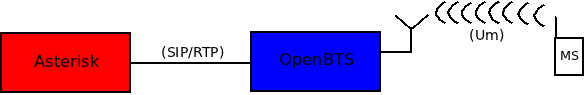
\includegraphics[width=0.80\textwidth]{img/openbts_sip_asterisk.png}
	\caption{Terminierung der SIP-Verbindung an OpenBTS}
	\label{fig:openbts_sip_asterisk}
\end{figure}

Die bereits oben erwähnte Komponente \textit{sipauthserve} ist dabei für die Registrierung der MS zuständig und trägt dazu  die Teilnehmer in die Datenbank \verb|sqlite3.db| ein.\\ 
Nachfolgend werden drei wesentliche GSM-Szenarien beschrieben, um das Zusammenspiel aus GSM- und SIP, wie in Abbildung \ref{fig:openbts_system_diagram} gezeigt, zu verdeutlichen:
\begin{itemize}
\item \textbf{Registrierung (Location Update)}\\
Wenn die MS eingeschaltet wird oder eine neue Location Area betritt, führt sie einen \textit{LOCATION UPDATE REQUEST} (LUR) aus. Zudem ist es möglich das die BTS die MS periodisch dazu auffordert ein LUR auszuführen. Bei OpenBTS wird ein GSM LUR in Form eines \textit{SIP REGISTER} durchgeführt (siehe Abb. \ref{fig:openbts_registration}). Zuerst findet der allgemeine GSM Ablauf der Kanalanforderung (ausgehend von der MS) statt. Nun folgt das eigentliche Location Update. Dazu schickt die MS einen \textit{LOCATION UPDATE REQUEST} an OpenBTS, welche daraufhin ein \textit{SIP REGISTER} an \textit{sipauthserve} sendet. \textit{sipauthserve} erstellt nun einen entsprechenden Eintrag in der SQL-DB \verb|sqlite3.db| (siehe Abb. \ref{fig:openbts_system_diagram}). Zum Schluss wird der zugewiesene GSM Kanal wieder abgebaut. Von nun an ist die MS im Netz registriert und kann durch einen \textit{PAGING REQUEST} "`angesprochen"' werden.
\begin{figure}[h]
	\centering
		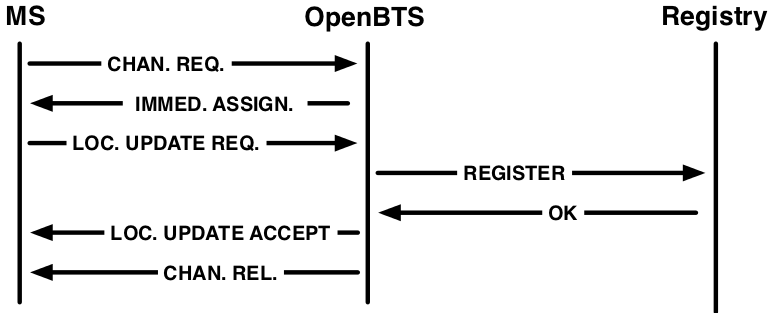
\includegraphics[width=0.80\textwidth]{img/openbts_registration.png}
	\caption{Location Update in Form eines SIP REGISTER (Quelle: \cite{bib:openbtsmanual}(S.47))}
	\label{fig:openbts_registration}
\end{figure}
\end{itemize}
\begin{itemize}
\item \textbf{Gesprächsaufbau (MS $\rightarrow$ SIP-Switch)}\\
Der Gesprächsaufbau ausgehend von der Mobile Station ist in Abbildung \ref{fig:openbts_call_msside} beschrieben. Die MS beantragt als erstes einen Kanal bei der BTS (\textit{CHANNEL REQUEST} auf \textit{RACH}), die BTS weist der MS daraufhin einen freien Kanal zu (\textit{IMMEDIATE ASSIGNMENT}), woraufhin dann diese eine Anfrage zum Verbindungsaufbau (\textit{CM SERVICE REQUEST}) an die BTS sendet. Akzeptiert die BTS die Anforderung, so folgt nun der eigentliche Aufbau des Gesprächs (\textit{SETUP}). OpenBTS sendet dazu einerseits einen \textit{SIP INVITE} an die PBX um eine SIP Session aufzubauen, und andererseits ein \textit{CALL PROCEEDING} zur Signalisierung an die MS. Wenn die SIP-Gegenstelle erreichbar ist (\textit{Status: 200 OK}) bekommt die MS dies als Läutezeichen (\textit{ALERTING}) mitgeteilt. Nimmt zudem die Gegenstelle das Gespräch an, so ist der Verbindungsaufbau komplett. Zwischen OpenBTS und PBX besteht nun eine RTP-Verbindung über die die Sprachpakete transportiert werden, und zwischen OpenBTS und MS besteht eine herkömmliche Sprachverbindung (\textit{TCH}) auf der GSM Luftschnittstelle.
\begin{figure}[h]
	\centering
		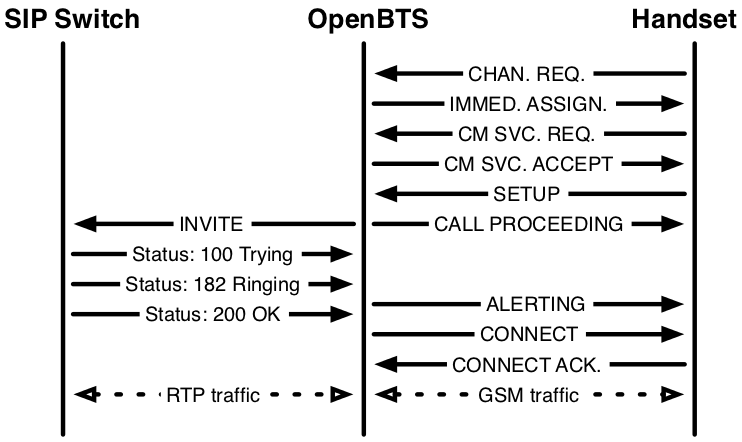
\includegraphics[width=0.80\textwidth]{img/openbts_call_msside.png}
	\caption{Gespräch ausgehend von der Mobile Station (Quelle: \cite{bib:openbtsmanual}(S.48))}
	\label{fig:openbts_call_msside}
\end{figure}
\end{itemize}
\begin{itemize}
\item \textbf{Gesprächsaufbau (SIP-Switch $\rightarrow$ MS)}\\
Zur Vollständigkeit sei in Abbildung \ref{fig:openbts_call_carrierside} der Gesprächsaufbau ausgehend vom SIP-Switch erwähnt. Diesmal kommt der \textit{SIP INVITE} von der PBX aus. OpenBTS versucht nun die MS zu erreichen (\textit{PAGING REQUEST}). Bei Erfolg fordert die MS wiederum einen Kanal bei der BTS an (siehe Punkt vorher), dass GSM Gespräch wird aufgebaut (\textit{SETUP}) und falls der MS-Benutzer nun endgültig das Gespräch annimmt, ist der Verbindungsaufbau komplett. Nun besteht wieder eine RTP-Verbindung zwischen PBX und OpenBTS, und eine Sprachverbindung (\textit{TCH}) auf der GSM Luftschnittstelle zwischen OpenBTS und MS. 
\begin{figure}[h]
	\centering
		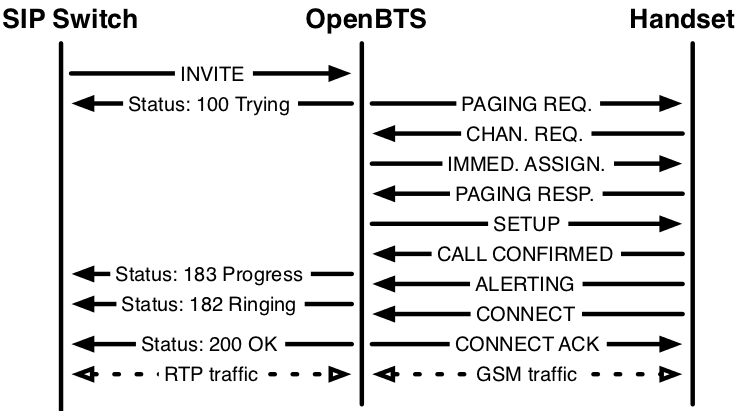
\includegraphics[width=0.80\textwidth]{img/openbts_call_carrierside.png}
	\caption{Gespräch ausgehend vom SIP-Carrier (Quelle: \cite{bib:openbtsmanual}(S.48))}
	\label{fig:openbts_call_carrierside}
\end{figure}
\end{itemize}

\subsection{Installation}
\label{sec:Installation}
Die Installation von \textbf{GNUradio, OpenBTS samt smqueue und sipauthserve}, sowie \textbf{Asterisk} erfolgte auf einem Ubuntu Linux 10.04.2 LTS. Dabei wurden die folgende Schritte bei der Installation des jeweiligen Softwarepakets durchgeführt.\\

\begin{center}
\begin{tabular}{l|l}
\textbf{Paket} & \textbf{Version}\\
\hline 
GNUradio & 3.4.2\\
OpenBTS & P2.8 (SVN)\\
smqueue & P2.8 (SVN)\\
sipauthserve & P2.8 (SVN)\\
Asterisk & 1.6.2.9 (Ubuntu Repository)\\
\end{tabular}
\end{center}
\textit{Auf Paketabhängigkeiten wurde größtenteils Rücksicht genommen. Sollte es trotzdem zu ungelösten Abhängigkeiten kommen, so können fehlende Pakete bspw. mittels} \verb|apt-get| \textit{aus entsprechenden Distributions-Repositories nachinstalliert werden.}

\subsubsection{GNUradio}
\textbf{GNUradio} wurde mit USRP1-Unterstützung kompiliert und installiert. 

\begin{enumerate}
	\item Fehlende Abhängigkeiten installieren:
	\begin{verbatim}
	sudo apt-get -y install git-core autoconf automake \
	libtool g++ python-dev swig pkg-config \
	libboost-all-dev libfftw3-dev libcppunit-dev \
	libgsl0-dev libusb-dev sdcc libsdl1.2-dev \
	python-wxgtk2.8 python-numpy python-cheetah \
	python-lxml doxygen python-qt4 python-qwt5-qt4 \
	libxi-dev libqt4-opengl-dev libqwt5-qt4-dev \
	libfontconfig1-dev libxrender-dev
	\end{verbatim}
	\item GNUradio mit USRP1-Unterstützung kompilieren und installieren:
	\begin{verbatim}
	wget http://gnuradio.org/redmine/attachments/\
	download/279/gnuradio-3.4.2.tar.gz
	tar xzf gnuradio-3.4.2.tar.gz
	cd gnuradio-3.4.2/
	./configure -with-usrp1
	make
	make check
	sudo make install
	\end{verbatim}
	\item Cache des Runtime Linkers aktualisieren:
	\begin{verbatim}
	export LD_LIBRARY_PATH=/usr/local/lib
	sudo ldconfig	
	\end{verbatim}
\end{enumerate}
 
\subsubsection{OpenBTS}
Für die Installation von \textbf{OpenBTS, smqueue und sipauthserve} wurde die aktuellste Version aus dem SVN-Repository verwendet.

\begin{enumerate}
	\item Fehlende Abhängigkeiten installieren:
	\begin{verbatim}
	sudo apt-get install autoconf libtool libosip2-dev \
	libortp-dev libusb-1.0-0-dev g++ sqlite3 \
	libsqlite3-dev erlang
	\end{verbatim}
	\item Sourcecode aus SVN-Repository kopieren:
	\begin{verbatim}
	mkdir openbts
	cd openbts
	svn co http://wush.net/svn/range/software/public
	\end{verbatim}
	\item In OpenBTS-Source-Verzeichnis wechseln und OpenBTS mit USRP1-Unterstützung kompilieren:
	\begin{verbatim}
	autoreconf -i
	./configure --with-usrp1
	make
	\end{verbatim}
	\item Da wir die USRP1 mit einem 52MHz Takt betreiben muss ein Link zur entsprechenden Transceiver-Binary erstellt, sowie die passende "`inband"'-Tabelle kopiert werden:
	\begin{verbatim}
	(from OpenBTS root)
	cd apps/
	ln -s ../Transceiver52M/transceiver .
	sudo mkdir -p /usr/local/share/usrp/rev4/
	sudo cp ../Transceiver52M/std_inband.rbf \
	/usr/local/share/usrp/rev4/
	cd ..
	\end{verbatim}
	\item Seit Version 2.8 wird die Konfiguration von OpenBTS nun nicht mehr in einzelnen großen Konfigurationsdatei gespeichert, sondern in einer SQL-Datenbank verwaltet. Diese erzeugen wir mit Hilfe des bereitgestellten Templates :
	\begin{verbatim}
	(from the OpenBTS directory)
	sudo mkdir /etc/OpenBTS
	sudo sqlite3 -init ./apps/OpenBTS.example.sql \
	/etc/OpenBTS/OpenBTS.db
	( .exit zum verlassen von sqlite3)
	\end{verbatim}
\end{enumerate}

\subsubsection{Subscriber Registry und Sipauthserve}
\begin{enumerate}
	\item Zuerst sollte \textbf{Asterisk} installiert werden damit die entsprechenden Verzeichnisse existieren:
	\begin{verbatim}
	sudo apt-get install asterisk
	\end{verbatim}
	\item Im SVN-Repository befindet sich ein SQL-Skript das nun für die Erstellung der Subscriber Registry benutzt wird:
	\begin{verbatim}
	(from svn root)
	cd public/subscriberRegistry/trunk/configFiles/
	sudo mkdir /var/lib/asterisk/sqlite3dir
	sudo sqlite3 -init subscriberRegistryInit.sql \
	/var/lib/asterisk/sqlite3dir/sqlite3.db
	( .exit zum verlassen von sqlite3)
	\end{verbatim}
	\item Nun wird \textbf{sipauthserve} kompiliert und dessen Konfigurationsdatenbank in \verb|/etc/OpenBTS/| erzeugt:
	\begin{verbatim}
	(from svn root)
	cd subscriberRegistry/trunk
	make
	sudo sqlite3 -init sipauthserve.example.sql \
	/etc/OpenBTS/sipauthserve.db
	( .exit zum verlassen von sqlite3)
	\end{verbatim}
\end{enumerate}

\subsubsection{Smqueue}
\begin{enumerate}
	\item \textbf{Smqueue} kompilieren:
	\begin{verbatim}
	(from svn root)
	cd smqueue/trunk/
	autoreconf -i
	./configure
	make
	\end{verbatim}
	\item Konfigurationsdatenbank von smqueue in \verb|/etc/OpenBTS/| erzeugen
	\begin{verbatim}
	sudo sqlite3 -init smqueue/smqueue.example.sql \
	/etc/OpenBTS/smqueue.db
	( .exit zum verlassen von sqlite3)
  \end{verbatim} 
\end{enumerate}

\subsection{Konfiguration}
\label{sec:Konfiguration}
\subsubsection{OpenBTS}
Die Datenbank \verb|/etc/OpenBTS/OpenBTS.db| enthält sämtliche Konfigurationsparameter für OpenBTS. Eine Liste aller Parameter, sowie dessen Beschreibung, findet man unter \url{https://wush.net/trac/rangepublic/wiki/openBTSConfig}.
Die Parameter können entweder direkt in der Datenbank \verb|OpenBTS.db| (z.B. mittels \verb|sqlite3 /etc/OpenBTS/OpenBTS.db|) oder am OpenBTS-Prompt mit den Befehlen \verb|config| bzw. \verb|unconfig| geändert werden.

Für die meisten Parameter eignen sich die bereits eingetragenen Standardwerte, jedoch sind einige grundlegende Einstellungen vorzunehmen:

\begin{itemize}
  \item \textbf{GSM.Radio.Band}\\
  Bestimmt das benutzte GSM-Band, bei uns: \textbf{1800}
  \item \textbf{GSM.Radio.C0}\\
  Die ARFCN Nummer, bei uns: \textbf{867}
  \item \textbf{GSM.CellSelection.Neighbors}\\
  ARFCN der Nachbarzellen, bei uns: \textbf{846}
  \item \textbf{Control.LUR.OpenRegistration}\\
  Mittels eines regulären Ausdrucks werden die IMSIs definiert, die sich an der BTS registrieren dürfen. Für Testzwecke ist es jedoch sinnvoll eine offene Registrierung zu verwenden, d.h. es darf sich jede MS verbinden. Dazu ist der Wert auf \textbf{Null} zu setzen.
  \item \textbf{GSM.Identity.MCC}\\
  Der Mobile Country Code bestimmt ist die Länderkennung, bei uns: \textbf{262} für Deutschland.
  \item \textbf{GSM.Identity.MNC}\\
  Der Mobile Network Code ist eine zweistellige Nummer die den Mobilfunkanbieter kennzeichnet. In Deutschland besitzt T-Mobile beispielsweise die 01, E-Plus die 03 und O2 die 07. Wir haben den Wert \textbf{99} eingestellt, da sich dieser offiziell nicht in Gebrauch befindet.
  \item \textbf{GSM.Identity.ShortName}\\
  Kurze Bezeichnung des Netzwerks; wird bei manchen Mobilfunktelefonen im Display angezeigt (überwiegend neuere Modelle); bei uns \textbf{OpenBTS HM}
  \item \textbf{GSM.RACH.AC}\\
  Die Access Class Flags sollten bei einem nicht funktionstüchtigen Netz auf \verb|0x0400| gesetzt werden, um dem Benutzer mitzuteilen, dass keine Notrufunterstützung existiert.    
\end{itemize} 

\subsubsection{Sipauthserve}
In der Regel müssen keine weiteren Einstellungen vorgenommen werden, solang man den Standardpfad für die \verb|sqlite3.db| eingehalten hat. Hat man dies nicht, so ist der neue Dateipfad (Feld: \verb|SubscriberRegistry.db|) in der Konfigurationsdatenbank (\verb|/etc/OpenBTS/sipauthserve.db|) anzugeben. Hilfreich könnte auch das Hochsetzen des \verb|Log.Level| sein, welches standardmäßig auf \textit{WARNING} eingestellt ist und unter \textit{DEBUG} deutlich mehr Hinweise bzgl. der erstellten Registry-Einträge offenbart.

\subsubsection{Smqueue}
Auch an der Konfiguration von \textit{smqueue} muss zwangsläufig keine Änderung vorgenommen werden. Allerdings enthält die Konfigurationsdatenbank (\verb|/etc/OpenBTS/smqueue.db|) weitaus mehr Einträge als die von sipauthserve. Gut die Hälfte dieser Parameter beziehen sich auf die "`Short Code"'-Funktionalität.

\subsubsection{Asterisk}
Die Konfiguration von Asterisk beschränkt sich in diesem Dokument auf die Intra-BTS-Kommunikation, d.h. es können nur Gespräche zwischen MS und MS bzw. MS und Asterisk-Diensten (Echo-Test, VoiceMail) statt finden, nicht jedoch von oder nach Außerhalb (Festnetz, andere SIP-Teilnehmer) telefoniert werden.
\begin{itemize}
\item \textbf{Teilnehmereintrag}\\\label{asterisk_teilnehmer}Damit die MS untereinander telefonieren können, müssen die Asterisk-Konfigurationsdateien \verb|sip.conf| und \verb|extensions.conf| im Verzeichnis \verb|/etc/asterisk/| angepasst werden. Als Beispiel wird die \textbf{IMSI 001010000000000} verwendet und dieser die Teilnehmerrufnummer \textbf{2101} zugeordnet.\\

In \verb|sip.conf| muss folgender Eintrag hinzugefügt werden:
\newpage
\begin{figure}[ht]
\setbox0\vbox{\small
\begin{verbatim}

...
[IMSI001010000000000]
callerid=2101         ; Teilnehmerrufnummer (diese
                      ; sieht auch die Gegenstelle)
canreinvite=no        ; Asterisk ist Mittelsmann
                      ; zwischen MS und Gegenstelle
type=friend           ; MS ruft uns bzw. wir rufen MS an
context=sip-external  ; zugeordneter Kontext
allow=gsm             ; Sprachcodec 'gsm' erlauben
host=dynamic          ; dynamischer Hostname
dtmfmode=rfc2833      ; DTMF-Töne nach Standard RFC2833
...
\end{verbatim}
}
\centerline{\fbox{\box0}}
\end{figure}

In \verb|extensions.conf| muss je IMSI ein Eintrag in der ihr zugeordneten Extension (hier \verb|sip-external|) hinzugefügt werden:
\begin{figure}[ht]
\setbox0\vbox{\small
\begin{verbatim}

...
[sip-external]
exten => 2101,1,Dial(SIP/IMSI001010000000000@127.0.0.1:5062)
...
\end{verbatim}
}
\centerline{\fbox{\box0}}
\end{figure}
\end{itemize}
\begin{itemize}
\item \textbf{Echo-Test}\\Zu Testzwecken empfiehlt es sich einen sog. "`Echo-Test"' unter Asterisk zu konfigurieren. Bei einem Echo-Test wird alles was man sagt als Echo zurückgeschickt. Zum einen erkennt man dadurch welche Latenzzeit zwischen MS und Asterisk besteht und zum anderen lässt sich ein Sprachkanal ohne die Notwendigkeit einer zweiten MS einfach aufbauen.
Um den Echo-Test zu aktivieren, werden folgende Zeilen in die \verb|extensions.conf| innerhalb des Kontext \verb|[sip-external]| eingefügt:
\begin{figure}[ht]
\setbox0\vbox{\small
\begin{verbatim}

[sip-external]
...
exten => 600,1,Answer()
exten => 600,2,Playback(demo-echotest)
exten => 600,3,Echo()
exten => 600,4,Playback(demo-echodone)
exten => 600,5,Hangup()
...
\end{verbatim}
}
\centerline{\fbox{\box0}}
\end{figure}

Nun ist der Echo-Test unter der Rufnummer 600 zu erreichen.\\

In der Praxis zeigte sich, dass die Sprachverzögerung um die 0.5 Sekunden liegt, was mit hoher Wahrscheinlichkeit an OpenBTS liegt. Ein zweiter Test zwischen Asterisk und einem herkömmlichen SIP-Client (Software), über eine direkte VoIP-Verbindung, wies nämlich keine nennenswerte Latenz auf.
\end{itemize}
\begin{itemize}
\item \textbf{VoiceMail}\\Jedem eingetragenen Teilnehmer kann eine Mailbox zugeordnet werden, welche aktiv wird wenn der Teilnehmer entweder nicht erreichbar ist (im Netz nicht registriert) oder nach einer einstellbaren Zeit den Anruf nicht entgegennimmt.
Für die Einrichtung einer Mailbox sind die folgende Schritte notwendig:
\begin{enumerate}
\item Neuen Kontext und Benutzer in \verb|/etc/asterisk/voicemail.conf| hinzufügen:
\begin{figure}[ht]
\setbox0\vbox{\small
\begin{verbatim}

...
[mailbox]
2101 => 1234, 2101		; #Rufnummer => #Passwort, #Benutzer
;weitere VoiceMail-Benutzer
...
\end{verbatim}
}
\centerline{\fbox{\box0}}
\end{figure}
\item Regelwerk in \verb|/etc/asterisk/extensions.conf| anpassen und VoiceMail-Abfrage hinzufügen:
\begin{figure}[ht]
\setbox0\vbox{\small
\begin{verbatim}

...
[sip-external]
exten => 2101,1,Dial(SIP/IMSI001010000000000
         @127.0.0.1:5062,20)
exten => 2101,2,VoiceMail(2101@mailbox)
exten => 2101,3,PlayBack(vm-goodbye)
exten => 2101,4,HangUp()

exten => 8888,1,VoiceMailMain(s${CALLERID(num)}@mailbox)	; Abfrage ohne Auth.
exten => 9999,1,VoiceMailMain(@mailbox)						; Abfrage mit Auth.
...
\end{verbatim}
}
\centerline{\fbox{\box0}}
\end{figure}

Das obige Regelwerk des Benutzers mit der Teilnehmerrufnummer 2101 besagt folgendes:\\
Zuerst wird versucht den Benutzer \textbf{IMSI001010000000000} über SIP zu erreichen (siehe Kapitel \ref{gsmsip}). Falls er im Netz registriert ist und die MS über \textit{PAGING} erreichbar ist, wird man nun maximal 20 Sekunden lang anläuten und nach Ablauf dieser Zeit zu Regel 2 springen. Ist der Benutzer erst gar nicht im Netz registriert, so wird unmittelbar zu Regel 2 gesprungen. Regel 2 definiert den eigentlichen Mailbox-Befehl. Der Anrufende hört die Mailboxansage und hat die Möglichkeit eine Nachricht zu hinterlassen. Hat er dies getan, so kann er entweder direkt auflegen oder mittels der Rautetaste die Aufnahme beenden. Regel 3 spielt daraufhin ein "`Auf wiedersehen"'-Soundfile ab und Regel 4 beendet letztendlich den Anruf.

Zur Mailbox-Abfrage hat man zwei Möglichkeiten. Ruft man, in unserem Beispiel, die Nummer \textbf{8888} an, so gelangt man direkt, d.h. ohne interaktive Authentifizierung, zu seinem Mailbox-Menü. Dort kann man aufgenommene Nachrichten abspielen, verwalten, löschen und weitere Mailbox-Optionen treffen. Unter der \textbf{9999} muss man sich erst mit seiner Mailbox-Kennung (hier im Beispiel ist das die 2101) und seinem Passwort (1234) gegenüber der Mailbox-Abfrage authentifizieren.

In der Praxis kam es zu Problemen bei der interaktiven Mailbox-Abfrage. Die Kennung und/oder das Passwort wurden als falsch von Asterisk betrachtet und eine erfolgreiche Authentifizierung war nicht möglich. Der Grund hierfür dürfte an einem nicht unterstützten bzw. nicht konfigurierten DTMF-Modus liegen, mittels dem die Tasteneingabe (Tastentöne) übertragen werden. Aus Zeitgründen und weil die Mailbox-Abfrage für unser Projektziel nicht relevant war, wurde der Sache nicht weiter auf den Grund gegangen.
\end{enumerate}
\end{itemize} 

\subsection{Benutzung von OpenBTS}
\subsubsection{Start der Dienste}
Damit die Registrierung der Teilnehmer und der Versand von Textnachrichten möglich ist, müssen neben OpenBTS auch die beiden Dienste \verb|sipauthserve| sowie \verb|smqueue| gestartet werden.
\begin{verbatim}
(from svn root)
./smqueue/trunk/smqueue/smqueue &
./subscriberRegistry/trunk/sipauthserve &
./openbts/trunk/apps/OpenBTS
\end{verbatim}

\subsubsection{Registrierung einer MS an OpenBTS}
Mit Hilfe der bereitgestellten Mobiltelefone vom Typ "`Nokia 3330"' und der programmierbaren SIM-Karten von Giesecke \& Devrient konnte nun eine Registrierung in unserem GSM Testnetz namens "`OpenBTS HM"' stattfinden. Dank der offenen Registrierung (\verb|Control.LUR.OpenRegistration|) kann man sich einfach am Netz registrieren und erhält zudem eine SMS, dessen Inhalt über den Konfigurationsparameter \verb|Control.LUR.OpenRegistration.Message| bestimmbar ist. Wichtiger Bestandteil dieser Kurzmitteilung ist die IMSI der SIM-Karte mit der sich die MS an der BTS registriert hat. Nun kann ein Teilnehmereintrag in Asterisk, wie in Kapitel \ref{asterisk_teilnehmer} beschrieben, erfolgen.\\
Folgendes Beispiel zeigt den SMS-Inhalt für die IMSI 262071111111111:
\begin{figure}[ht]
\setbox0\vbox{\small
\begin{verbatim}
Welcome to the GSM test network. Your IMSI is
IMSI:262071111111111
\end{verbatim}
}\centerline{\fbox{\box0}
}
\end{figure}

\subsubsection{Command Line Interface (CLI)}
Konnte OpenBTS erfolgreich gestartet werden, sieht man nun das Command Line Interface (CLI) vor sich:
\begin{figure}[ht]
\setbox0\vbox{\small
\begin{verbatim}
OpenBTS>
\end{verbatim}
}\centerline{\fbox{\box0}
}
\end{figure}\\
Nachfolgend einige Beispiele von hilfreichen CLI-Befehlen:
\begin{itemize}
\item \textbf{Befehl:} \verb|calls|\\
Listet aktive Gesprächs- bzw. SMS-Aktivitäten auf.
\begin{figure}[ht]
\setbox0\vbox{\small
\begin{verbatim}
OpenBTS> calls
2060207953 C0T1 TCH/F IMSI=001010000000000 L3TI=8 
SIP-call-id=1811340387 SIP-proxy=127.0.0.1:5060 MOC
to=600 GSMState=active SIPState=Active (5 sec)
\end{verbatim}
}\centerline{\fbox{\box0}
}
\end{figure}\\
Dabei ist \verb|2060207953| die Transaktions-ID, \verb|C0T1| die C0-ARFCN und der dabei verwendete Zeitschlitz (\textit{Nr. 1}), \verb|TCH/F| die Kanalart (\textit{Full-Rate Traffic Channel}) und \verb|IMSI=001010000000000| die IMSI des Teilnehmers. Die restlichen Angaben beziehen sich auf die SIP-Verbindung (\textit{ID, SIP-Status und Verbindungsdauer}).
\end{itemize}
\newpage
\begin{itemize}
\item \textbf{Befehl:} \verb|chans|\\
Listet aktive Kanäle und die dazugehörigen Leistungswerte auf.
\begin{figure}[ht]
\setbox0\vbox{\small
\begin{verbatim}
OpenBTS> chans
CN TN chan     transaction UPFER RSSI TXPWR TXTA DNLEV DNBER
CN TN type     id          pct    dB   dBm  sym   dBm   pct
 0 1    TCH/F  1247828231  0.54  -53    30    1   -48  0.00
\end{verbatim}
}\centerline{\fbox{\box0}
}
\end{figure}\\
Im obigen Beispiel handelt es sich um einen Verkehrskanal im Full-Rate Modus (\verb|TCH/F|) der den ersten Zeitschlitz (\verb|TN=1|) belegt und der Transaktions-ID \verb|1247828231| zugeordnet ist. Die MS sendet mit \verb|30 dBm| (\verb|TXPWR|) und besitzt einen Timing Advance (\verb|TXTA|) Wert von \verb|1|. Die beiden Angaben \verb|UPFER| und \verb|RSSI| beziehen sich auf den Uplink. \verb|UPFER| gibt dabei die Fehlerrate der Frames an, die im Beispiel bei \verb|0,54| Prozent liegt, und \verb|RSSI| die Stärke des Sendesignals der MS, hier \verb|-53 dBm|. Für den Downlink gibt \verb|DNBER| die Fehlerrate der Bits an und \verb|DNLEV|, dass Pendant zu RSSI im Uplink, gibt die Empfangssignalstärke der MS, hier \verb|-48 dBm|, an.
\end{itemize}
\begin{itemize}
\item \textbf{Befehl:} \verb|tmsis|\\
Listet die aktuelle TMSI-Tabelle auf.
\begin{figure}[ht]
\setbox0\vbox{\small
\begin{verbatim}
OpenBTS> tmsis
TMSI       IMSI             age   used
1          001010000000000  138s  138s
\end{verbatim}
}\centerline{\fbox{\box0}
}
\end{figure}\\
Im Beispiel wurde der IMSI \verb|001010000000000| die TMSI \verb|1| zugeordnet. Dieser Eintrag wurde vor 138s (\verb|age|) erstellt. Ebenfalls 138s ist diese TMSI in Gebrauch (\verb|used|). 
\end{itemize}

Eine Liste aller möglichen OpenBTS-Befehle sowie dessen Beschreibung findet sich unter \url{https://wush.net/trac/rangepublic/wiki/cli} oder im Benutzerhandbuch von OpenBTS \cite{bib:openbtsmanual}(Kapitel 5.5).



\section{Erweiterung von OpenBTS}
\utsubsection{Measurement Report}{Max Eschenbacher}
Measurement Reports enthalten Messwerte bzgl. der Empfangsleistung, Empfangsqualität und Informationen zu Nachbarzellen. Sie werden beim Einbuchen in das Netzwerk und während eines Gesprächs (ca. 2 mal in der Sekunde) von der MS an die BTS gesandt. Measurement Reports sind im RR-Sublayer (Radio Resource) angesiedelt und mit dem Nachrichtentyp \textit{MEASUREMENT REPORT} gekennzeichnet. Die Messwerte sind für das Weiterreichen (Handover) der MS von großer Bedeutung.

OpenBTS verwaltet diese Messwerte intern in einer eigenen Klasse, bietet aber auch die Möglichkeit, diese in eine externe SQL-DB abzulegen. Mit der Option \verb|Control.Reporting.PhysStatusTable| kann der Pfad der Datenbank angegeben werden:
\begin{verbatim}
OpenBTS> config Control.Reporting.PhysStatusTable \
/etc/OpenBTS/phystatus.db
\end{verbatim}

Leider werden keinerlei Informationen bzgl. der Nachbarzellen in die Datenbank eingetragen. Deshalb musste die entsprechende Tabelle der Datenbank um weitere Felder für die Nachbarzellen erweitert und die Methode \verb|PhysicalStatus::setPhysical()| angepasst werden.
Zusätzlich wurde ein neuer CLI-Befehl namens \verb|showmr| implementiert, welcher den Inhalt der Measurement Report DB entsprechend formatiert und auflistet.

\newpage
Beispielausgabe von \verb|showmr|:
\begin{figure}[ht]
\setbox0\vbox{\small
\begin{verbatim}
OpenBTS> showmr
############################################################
                Measurement Report:
############################################################
CN_TN_TYPE_OFFSET               =       C0T0 SDCCH/4-0
ARFCN                           =       867
ACCESSED                        =       1330702677
RSSI                            =       -63.750000
TIME_ERR                        =       -0.222656
TIME_ADVC                       =       1
TRANS_PWR                       =       30 dBm
FER                             =       0.000000
RXLEV_FULL_SERVING_CELL         =       -48 dBm
RXLEV_SUB_SERVING_CELL          =       -48 dBm
RXQUAL_FULL_SERVING_CELL_BER    =       0.181000 dBm
RXQUAL_SUB_SERVING_CELL_BER     =       0.181000 dBm
NO_NCELL                        =       1
RXLEV_CELL_1 = 0, BCCH_FREQ_CELL_1 = 0, BSIC_CELL_1 = 0
RXLEV_CELL_2 = 0, BCCH_FREQ_CELL_2 = 0, BSIC_CELL_2 = 0
RXLEV_CELL_3 = 0, BCCH_FREQ_CELL_3 = 0, BSIC_CELL_3 = 0
RXLEV_CELL_4 = 0, BCCH_FREQ_CELL_4 = 0, BSIC_CELL_4 = 0
RXLEV_CELL_5 = 0, BCCH_FREQ_CELL_5 = 0, BSIC_CELL_5 = 0
RXLEV_CELL_6 = -33, BCCH_FREQ_CELL_6 = 63, BSIC_CELL_6 = 1
############################################################
CN_TN_TYPE_OFFSET               =       C0T1 TCH/F
ARFCN                           =       867
ACCESSED                        =       1330696371
RSSI                            =       -57.250000
TIME_ERR                        =       0.263672
TIME_ADVC                       =       1
TRANS_PWR                       =       30 dBm
FER                             =       0.042869
RXLEV_FULL_SERVING_CELL         =       -48 dBm
RXLEV_SUB_SERVING_CELL          =       -48 dBm
RXQUAL_FULL_SERVING_CELL_BER    =       0.000000 dBm
RXQUAL_SUB_SERVING_CELL_BER     =       0.000000 dBm
NO_NCELL                        =       7
RXLEV_CELL_1 = 0, BCCH_FREQ_CELL_1 = 0, BSIC_CELL_1 = 0
RXLEV_CELL_2 = 0, BCCH_FREQ_CELL_2 = 0, BSIC_CELL_2 = 0
RXLEV_CELL_3 = 0, BCCH_FREQ_CELL_3 = 0, BSIC_CELL_3 = 0
RXLEV_CELL_4 = 0, BCCH_FREQ_CELL_4 = 0, BSIC_CELL_4 = 0
RXLEV_CELL_5 = 0, BCCH_FREQ_CELL_5 = 0, BSIC_CELL_5 = 0
RXLEV_CELL_6 = 0, BCCH_FREQ_CELL_6 = 0, BSIC_CELL_6 = 0

############################################################
\end{verbatim}
}
\centerline{\fbox{\box0}}
\end{figure}
\newpage

\underline{Erläuterungen zur Beispielausgabe}

Der erste Measurement Report wurde um \verb|1330702677| (Unix-Time, entspricht 02.03.2012 - 16:37:57 Realzeit) im \verb|SDCCH| (\textit{Standalone Dedicated Control Channel}) mit der Nummer 0 (von 4 Möglichen) auf der \verb|ARFCN 867| gesendet. Die empfangene Signalstärke (\verb|RSSI = Received Signal Strength Indication|) betrug \verb|-63.75 dBm|. Der zugeordnete Timing Advance Parameter der MS betrug 1 Symbolperiode und wies einen Fehler (\verb|TIME_ERR|), d.h. Zeitversatz von \verb|-0.222656| Symbolperioden auf. Die Sendeleistung der MS betug \verb|30 dBm| und hatte bis dato eine \verb|Uplink-FER| (= Frame Erasure Rate; gibt das Verhältnis zwischen gelöschten Frames und der Gesamtanzahl der Frames an) von \verb|0|. Der Empfangspegel der verwendeten Zelle (\verb|RXLEV_FULL_SERVING_CELL|) betrug \verb|-48 dBm| und die Empfangsqualität \verb|RXQUAL_FULL_SERVING_CELL_BER = 0.181000 dBm|. Die Angaben \verb|SUB| und \verb|FULL| bei der Empfangsleistung und -qualität beziehen sich auf die Verwendung von DTX (Discontinuous Transmission). \verb|FULL| bezieht dabei alle Frames mit ein, also auch die zu dessen Zeit keine Sprache gesendet wurde. \verb|SUB| hingegen nur die effektiven "`Sprachframes"'. Da jeweils beide Werte im obigen Beispiel gleich sind, kann man davon ausgehen das kein DTX verwendet wurde. Die restlichen Angaben beziehen sich auf die Nachbarzellen. \verb|NO_NCELL| gibt die Anzahl der sichbaren Nachbarzellen an. Dabei gibt es zwei Sonderfälle: \verb|NO_NCELL=0| - es existieren keine Messwerte, \verb|NO_NCELL=7| - es existieren keine Nachbarzellen. Im obigen Beispiel sieht die MS 1 Nachbarzelle (Nr. 6) mit einer Empfangsleistung von \verb|-33 dBm|. 

\utsubsection{Handover-Modul}{Stefan Giggenbach}\label{sec:hom}

Das implementierte Handover-Modul muss im Prinzip die am Ende des Abschnitts \ref{sec:handover} beschriebenen Aufgaben abarbeiten. Die Erfassung der Measurement Reports wurde bereits in Abschnitt \ref{sec:measrep} beschrieben. Dabei wird, wie bereits erwähnt, nicht die vorhandene SQLite3-Datenbank, sondern zwei neu erstellte Klassen, deren Klassendiagramme in Abbildung \ref{fig:homclass} dargestellt sind, verwendet. Die Definition und Implementierung befindet sich in den Dateien \lstinline{GSMHandover.h} und \lstinline{GSMHandover.cpp} des \textit{GSM}-Moduls.

\begin{figure}[h!t!b!p!]
  \centering
  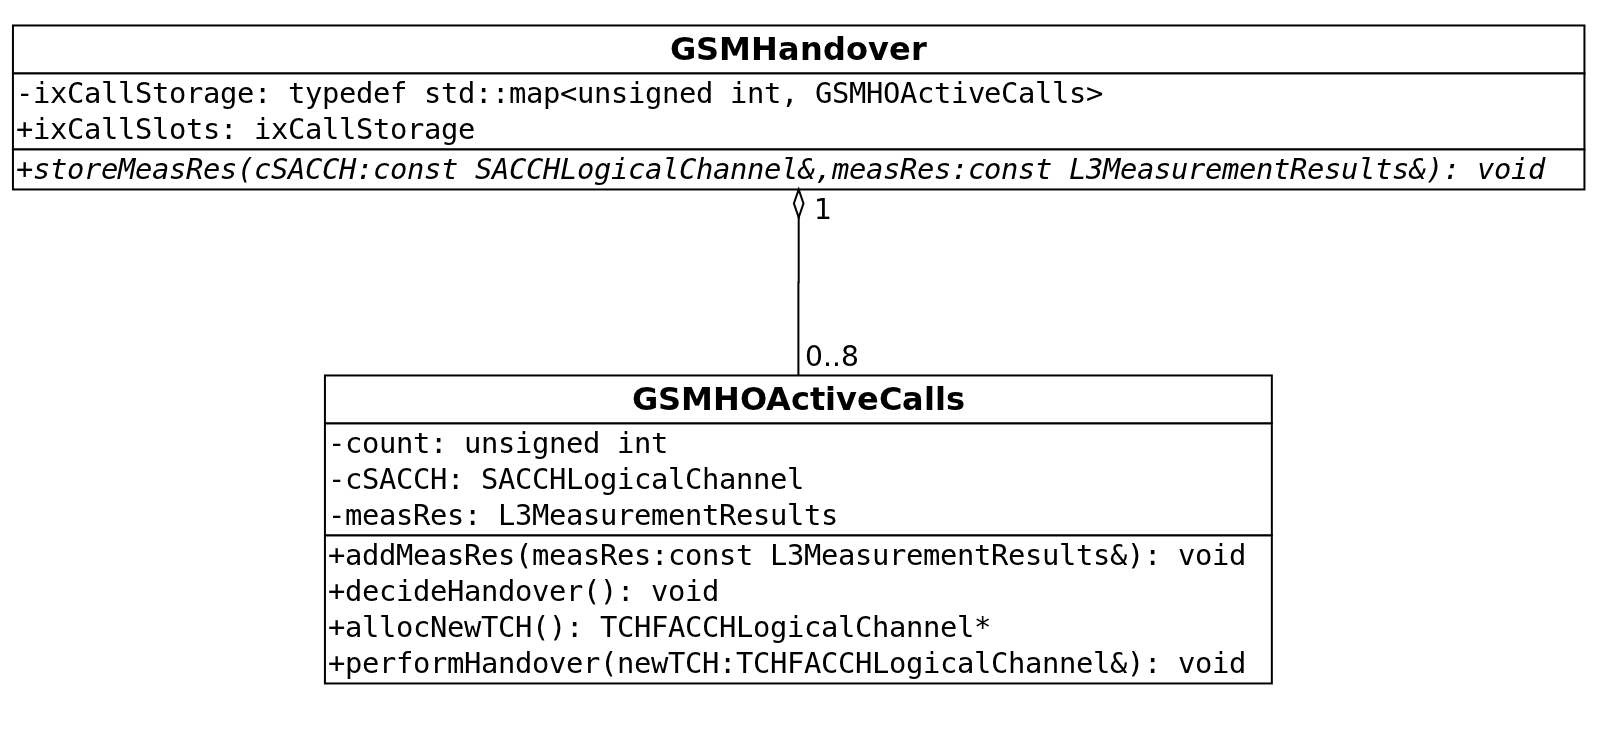
\includegraphics[width=0.8\textwidth]{img/homc}
  \caption{Klassendiagramm Handover-Modul}
  \label{fig:homclass}
\end{figure}

Von der Klasse \lstinline{GSMHandover} wir in der Datei \lstinline{OpenBTS.cpp} des \textit{apps}-Moduls ein globales Objekt instanziiert. Nach dem schreiben der aktuellen Measurement Reports in die SQLite3-Datenbank wird die Methode \lstinline{storeMeasRes()} des \lstinline{GSMHandover}-Objekts aufgerufen. Der Methode werden als Parameter die Referenz auf ein \lstinline{L3MeasurementResults}-Objekt und eine Referenz auf das entsprechende \lstinline{SACCHLogicalChannel}-Objekt übergeben. Mit Hilfe der Frequenz und des Timeslots des \gls{sacch} werden bis zu acht Objekte des Typs \lstinline{GSMHOActiveCalls} in der Map des \lstinline{GSMHandover}-Objekts verwaltet und die neusten Measurement Reports entsprechend zugeordnet.

Die Abarbeitung der restlichen in Abschnitt \ref{sec:handover} beschriebenen Aufgaben erfolgt mit Hilfe der Methoden der Klasse \lstinline{GSMHOActiveCalls}. Die Methode \lstinline{addMeasRes()} überschreibt dabei lediglich das in der Membervariablen gespeicherte Messergebnis. Hier wären zusätzliche Erweiterungen wie die speicherung von beispielsweise bis zu zehn Messergebnissen und die Bildung eines gleitenden Mittelwerts denkbar.

Die Methode \lstinline{decideHandover()} ist für die logische Entscheidungsfindung der Notwendigkeit eines Handover zuständig. In der aktuellen Implementierung prüft die Methode lediglich das vorhandensein der Datei \lstinline{doit} im aktuellen Arbeitsverzeichnis. Auf diese Art kann mit der Eingabe von \lstinline{touch doit} in einer Shell ein Handover manuell für Testzwecke ausgelöst werden. In Zukunft sollte diese Methode die Messergenisse von verscheidenen BTS berücksichtigen und eine logische Entscheidung treffen.

Für den Aufbau eines neuen TCH in einer benachbarten BTS ist eine Kommunikation zwischen den beiden System notwendig. Normalerweise erledigt diese Aufgabe der BSC. Im Fall von OpenBTS diese Kommunikation erst implementiert werden. Diese aufwändige Arbeit konnte im Rahmen der Projektarbeit allerdings nur theoretisch ausgearbeitet werden (siehe Abschnitt \ref{sec:interbts}). Aus diesem Grund wird in der Methode \lstinline{allocNewTCH()} ein TCH innerhalb des aktiven OpenBTS Systems geöffnet.

Der Methode \lstinline{performHandover()} wird als Parameter die Referenz auf den neu allozierten TCH übergeben. Anschließend wird das in Kapitel \ref{sec:swarch} beschriebene Handover-Command erzeugt und über den bestehenden FACCH an die Mobile Station gesendet. Das Umschalten der SIP-Verbindung wäre ein wichtiger Zwischenschritt, der in der aktuellen Implementierung nicht enthalten ist. Neben der Inter BTS Kommunikation, ist diese Aufgabe eine Ansatzpunkt für zukünftige Projektgruppen. Nachdem dem Senden des Handover-Command wir der alte TCH mit Hilfe der entsprechenden GSM-Primitive freigegeben.

Dieser Intra BTS Handover wurde in mehrer Tests erfolgreich durchgeführt und konnte bereits wie in Kapitel \ref{sec:analyse} beschrieben getraced und analysiert werden.

\utsubsection{Inter OpenBTS Handover}{Thomas Waldecker}\label{sec:interbts}

Dieser Abschnitt beschreibt die theoretische Umsetzung eines Inter OpenBTS Hand\-overs. Als Vorraussetzung wird angenommen das eine OpenBTS Basisstation seine Benachbarten OpenBTS Basisstationen kennt. Alle OpenBTS sind mit einem Asterisk Server verbunden. Die Basisstationen können sich untereinander per IP erreichen. Ist jetzt ein Anruf aktiv auf einer Mobilstation und entscheidet die Basisstation das sie einen Handover durchführen möchte, führen die beiden Basisstationen einen peer-to-peer Handover durch, wobei die aktuelle Basisstation die Masterbasisstation ist.

\begin{figure}[htbp]
	\centering
		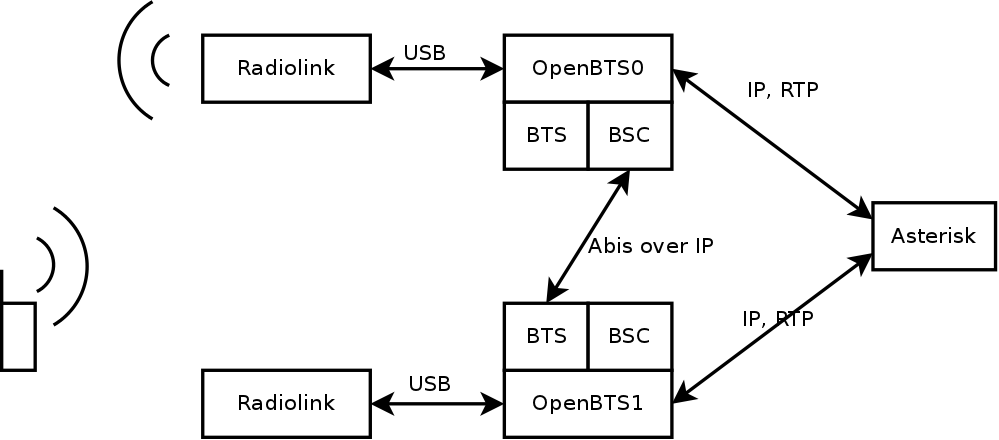
\includegraphics[width=0.9\textwidth]{img/inter_openbts}
	\caption{Kommunikation zwischen den Komponenten}
	\label{fig:interopenbts_komm}
\end{figure}

Sieht man die aktuelle Basisstation als BSC mit BTS und die neue OpenBTS Basisstation als reine BTS an, so wäre das Handoverszenario vergleichbar mit einem Intra BSC Handover.

Eine Weiterleitung des Sprachkanals kann entweder im Asterisk erfolgen oder von der origin OpenBTS zur neuen OpenBTS weitergeleitet werden. 

\utsection{Analyse}{Thomas Waldecker}\label{sec:analyse}

\subsection{Vorbereitung}
\subsubsection{Tracen auf dem Um Interface mit einem Nokia 3310}\label{sec:umtrace}
Das Um Interface kann mit einem Nokia 3310 Mobiltelefon und einem dazugehörigen Adapter, der zwischen den Akku und das Telefon gesteckt wird und auf die vier Kontakte des internen Telefonbus zugreift getraced werden.

Im Adapterkabel ist ein USB-zu-Seriell Wandler integriert. In die Konfigurationsdatei muss deshalb das Device des USB-Seriell Wandlers eingetragen werden (Siehe Listing \ref{config:gammu}).

\begin{lstlisting}[label=config:gammu,caption={Konfigurationsdatei für gammu und dem verwendeten Adapter}]
[gammu]

port = /dev/ttyUSB0
model = 6110
connection = mbus
synchronizetime = yes
logfile = 
logformat = nothing
use_locking = yes
gammuloc = 
\end{lstlisting}

Das Tracen kann nach der weiteren Konfiguration, die in \cite{bib:nokiagammu} beschrieben ist mit folgenden Kommando gestartet werden (Listing \ref{command:gammu}).

\begin{lstlisting}[label=command:gammu,caption={Aufruf von Gammu}]
sudo gammu --nokiadebug nhm5_587.txt v20-25,v18-19
Debug Trace Mode -- wumpus 2003
Loading
Activating ranges:
  20-25 verbose=1
  18-19 verbose=1
Debug Trace Enabled
Press Ctrl+C to interrupt...
<1805> MDI:m2d/FROM_MCU_TO_FBUS
t=0002 nr=0f: D 05: 1e 0c 00 40 00 06 01 01 70 01 01 47 
<198E> MDI:d2m/FROM_FBUS_TO_MCU
t=0003 nr=10: D 8E: 1e 00 0c 7f 00 02 40 07 
\end{lstlisting}

\subsubsection{Abis over IP tracen mit Wireshark}\label{sec:abistrace}
Das Abis Interface zwischen den \gls{bts} und dem \gls{bsc} kann mit Wireshark getraced werden (Siehe Abbildung \ref{fig:openbscarch}). Dazu wird auf der Maschine auf der OpenBSC läuft Wireshark auf dem Ethernet-Interface gestartet.

Das Abis over IP Protokoll wird nicht von Wireshark unterstützt und aufgelöst. Dieses Feature steht aber als Patches für Wireshark vom OpenBSC Projekt zur Verfügung.

Die Patches für Wireshark liegen im Repository von OpenBSC. Die Doku im OpenBSC-wiki ist dafür nicht so hilfreich. Wenn man sich den Quelltext von OpenBSC holt sind im Verzeichnis \lstinline{wireshark/} verschiedene Patches die auf die SVN-Revision r38894 von Wireshark angewendet werden können. Damit werden verschiedene Features zu Wireshark hinzugefügt \cite{bib:wiresharkabis, bib:wiresharkabisreadme}.

Angewendet werden diese Patches mit folgendem Kommando (ausgeführt im Wireshark Quelltextverzeichnis auf SVN Revision r38894):
\begin{lstlisting}[caption={Patchen von Wireshark}]
$ patch -p1 < $OPENBSC_DIR/wireshark/0001-abis_oml.patch
$ patch -p1 < $OPENBSC_DIR/wireshark/0002-ericsson_rbs2409.patch
$ patch -p1 < $OPENBSC_DIR/wireshark/0003-lucent-hnb.patch
$ patch -p1 < $OPENBSC_DIR/wireshark/0004-rsl-ipaccess.patch
$ patch -p1 < $OPENBSC_DIR/wireshark/0005-rsl-hsl.patch
$ patch -p1 < $OPENBSC_DIR/wireshark/0006-abis_oml-hsl.patch 
\end{lstlisting}

\subsection{Intra BSC Handover mit OpenBSC und zwei nanoBTS}

\subsubsection{Aufbau und Durchführung}
In einem Raum (Mobile Netze Labor) wurde an zwei Ecken jeweils eine nanoBTS gelegt und per Ethernet mit dem Laborrechner verbunden. Auf dem Rechner wurde OpenBSC gemäß Kapitel \ref{sec:openbsc} konfiguriert. Durch hin und hergehen zwischen den beiden \gls{bts} während eines Anrufs soll das OpenBSC Handover auslösen.

Während des Handovers wurde das Um Interface (siehe Kapitel \ref{sec:umtrace}) und das Abis Interface (siehe Kapitel \ref{sec:abistrace}) getraced.

Abbildung \ref{fig:adhandover} zeigt das Ablaufdiagramm eines Handovers. in den Folgenden zwei Abschnitten werden die zwei Traces untersucht. 

\subsubsection{Ablauf Handover auf dem Um Interface}

Während eines Anrufs werden laufend \textit{Measurement Reports} an die \gls{bts} über den \gls{sacch} gesendet. Die \gls{bts} leitet die Reports an die \gls{bsc} weiter, die letzendlich auch die Entscheidung über einen Handover trifft. Ist diese Entscheidung getroffen wird an die Mobilstation ein Handover Command gesendet. Die Mobilstation führt dann den Handover aus indem sie der neuen \gls{bts} eine \gls{sabm} Nachricht sendet um eine Verbindung aufzubauen. Die BTS beantwortet den \gls{sabm} Request mit einem \gls{UA} \cite[3.4.4]{bib:3gpp0408}\cite[3.1.5]{bib:3gpp0408} \cite[1.7.4]{bib:grundkursmks}.

Listing \ref{lst:bschandovertrace} zeigt die relevanten Pakete des Handovers auf dem Um Interface.

\begin{lstlisting}[label=lst:bschandovertrace,caption={Übersicht über die gesendeten Pakete auf dem Um Interface},numbers=none]
No. Src Dest Protocol Length Info
271	MS	BTS  LAPDm	  23     U, func=UI(DTAP) (RR) Measurement Report 
284	BTS	MS   LAPDm	  23     I, N(R)=4, N(S)=2(DTAP) (RR) Handover Command 
292	MS  BTS  LAPDm    23     U P, func=SABM
297	BTS MS   LAPDm	  23     U F, func=UA
\end{lstlisting}

Im weiteren Teil dieses Abschnitts wird auf die am Handover beteiligten Nachrichten genauer eingegangen.

\textbf{System Information Type 2}
Damit die Mobilstation erfährt welche benachbarten Zellen relevant sind für die Messung der Signalstärke schickt die Basisstation ein System Information Type 2. Diese benachbarten Zellen müssen vorher im BSC konfiguriert werden. In Listing \ref{lst:sysinftype2} ist ein Auszug aus dem System Information Type 2 mit dem die Neighbour Cell Description mitgesendet wird. Dort sieht man die List of \glspl{ARFCN}

\begin{lstlisting}[label=lst:sysinftype2,caption={Nachbarzellen im System Information Type 2}]
Neighbour Cell Description - BCCH Frequency List
..0. .... = EXT-IND: The information element carries the complete BA (0)
...0 .... = BA-IND: 0
10.. 111. = Format Identifier: variable bit map (0x47)
List of ARFCNs = 846
\end{lstlisting}

\textbf{Measurement Report}
Im Measurement Report sind die Measurement Results enthalten. Die Spezifikation mit dem Layout und der Beschreibung der Results ist in \cite[10.5.2.20]{bib:3gpp0408}. In Listing \ref{lst:measurement-result} ist die Beschreibung eines per Wireshark getraceten Reports abgedruckt.

Der Inhalt der Measurement Results wird nun kurz erklärt. Das Feld \lstinline{RXLEV-FULL-SERVING-CELL} gibt die empfangene Signalstärke auf allen Slots an. Das Messergebnis ist gültig, das gibt uns das Feld \lstinline{MEAS-VALID} an. Der Wert im Feld \lstinline{NO-NCELL} gibt an, das wir ein Messergebnis für eine Nachbarzelle haben. Das Messergebnis für dei Nachbarzelle ist im Feld \lstinline{RXLEV-NCELL} \cite[Table 10.40]{bib:3gpp0408}.

\begin{lstlisting}[label=lst:measurement-result,caption={Measurement Result}]
351	0	MS	BTS	LAPDm	23	U, func=UI(DTAP) (RR) Measurement Report 
  GSM A-I/F DTAP - Measurement Report
    Measurement Results
    0... .... = BA-USED: 0
    .0.. .... = DTX-USED: DTX was not used
    ..10 0010 = RXLEV-FULL-SERVING-CELL: -77 <= x < -76 dBm (34)
    0... .... = 3G-BA-USED: 0
    .0.. .... = MEAS-VALID: The measurement results are valid
    ..10 0100 = RXLEV-SUB-SERVING-CELL: -75 <= x < -74 dBm (36)
    .000 .... = RXQUAL-FULL-SERVING-CELL: BER < 0.2%, Mean value 0.14% (0)
    .... 000. = RXQUAL-SUB-SERVING-CELL: BER < 0.2%, Mean value 0.14% (0)
    .... ...0  01.. .... = NO-NCELL-M: 1 neighbour cell measurement result (1)
    ..10 1101 = RXLEV-NCELL: 45
    0000 0... = BCCH-FREQ-NCELL: 0
    .... .111  111. .... = BSIC-NCELL: 63
\end{lstlisting}

\textbf{Handover Command}
Fällt der \gls{bsc} die Entscheidung für einen Handover dann sendet die Basisstation einen Handover Command in dem unter anderem die Frequenz des Kontrollkanals (\gls{BCCH} \gls{ARFCN}) und die Beschreibung des \gls{TCH/F}, bestehend aus dem Timeslot und der Frequenz \gls{ARFCN}.

\begin{lstlisting}[label=lst:handover-command,caption={Handover Command}]
DTAP Radio Resources Management Message Type: Handover Command (0x2b)
 Cell Description
  ..11 1... = NCC: 7
  .... .111 = BCC: 7
  BCCH ARFCN(RF channel number): 840
 Channel Description 2 - Description of the first channel, after time
  0000 1... = TCH/F + FACCH/F and SACCH/F
  .... .010 = Timeslot: 2
  111. .... = Training Sequence: 7
  ...0 .... = Hopping channel: No
  .... 00.. = Spare
  Single channel : ARFCN 840
 Handover Reference
  Handover reference value: 6
 Power Command and access type
\end{lstlisting}
  
{\LARGE Platz für SABM - UA}

\subsubsection{Handover auf der Abis Schnittstelle zwischen OpenBSC und den zwei nanoBTS}

Wie in Abbildung \ref{fig:adhandover} zu sehen ist bekommt der \gls{bsc} in unserem Fall OpenBSC von der \gls{bts} mit der aktiven Verbindung die Measurement Reports. Entscheidet sich der \gls{bsc} für einen Handover dann sendet er ein Channel Activation an die neue \gls{bts}. Diese allokiert einen neuen Kanal und antwortet dann mit einem Channel Activation Acknowledgement. Dann sendet der \gls{bsc} den Handover Command zur alten BTS. Sobald ein Established Indication von der neuen BTS eintrifft wird der Sprachkanal an die neue BTS umgeleitet. Am Ende wird der Kanal auf der alten BTS mit einem Channel Release freigegeben. Die BTS bestätigt dies mit einem Channel Release Acknowledgement. 

\begin{lstlisting}

\end{lstlisting}







\section{Zusammenfassung und Ausblick}


%% Beim Anhang gibt es eine Musterdatei, die 
%% ergänzt werden kann
\appendix
\section{Anhang}
\setcounter{section}{1}


%% einfache Aufz�hlung, kein BibTeX
\subsection{Literaturverzeichnis}
\renewcommand\refname{\vspace*{-2em}}

\begin{thebibliography}{}
\bibitem{bib:grundkursmks} Martin Sauter:
{\it Grundkurs Mobile Kommunikationssysteme},
Vieweg+Teubner Verlag, Wiesbaden 2011

\bibitem{bib:buildopenbsc} Building OpenBSC:
\url{http://openbsc.osmocom.org/trac/wiki/Building_OpenBSC}
Abgerufen am 09.03.2012

\bibitem{bib:ipaccess} ipaccess-config (Konfiguration der nanoBTS):
\url{http://openbsc.osmocom.org/trac/wiki/ipaccess-config}
Abgerufen am 09.03.2012

\bibitem{bib:diagramm:openbts} OpenBTS System Diagramm:
\url{https://wush.net/trac/rangepublic/attachment/wiki/BuildInstallRun/openbts_system_diagram.png},
Abgerufen am 03.03.2012

\bibitem{bib:openbtsmanual} Range Networks Inc.:
{\it OpenBTS P2.8 Users Manual Doc. Rev. 1},
Range Networks Inc. 2011

\bibitem{bib:nokiagammu} AirProbe Wiki - tracelog:
\url{https://svn.berlin.ccc.de/projects/airprobe/wiki/tracelog}, Abgerufen am 09.03.2012

\end{thebibliography}
\leereseite



%% Stichwortverzeichnis ausgeben.
%% falls nicht notwendig, die folgende Zeile loeschen
\printindex

\end{document}
